% ----------------------------------------------------------------------
\chapter{Codeanalyse}
% ----------------------------------------------------------------------

In Kapitel 2.2 werden all die erstellten Dateien diskutiert. Im Folgenden werden die Header-Datei und Cpp-datei detailliert analysiert.  
\par In der Header Datei gibt es nur 2 Teile, die durch die Zugriffskontrollen private slot und private begrenzt werden. Im ersten Bereich werden die allen Funktionsdeklarationen, wie in Kapitel 4.1 erwähnt, automatisch erstellt. Des Weiteren werden die Deklarationen der manuell erstellten Funktionen und Variablen in Cpp-Datei manuell im zweiten Teil erstellt.
\par Cpp-Datei wird in vier Gruppen, nämlich Initialisierung, Destruktor, Slots-Funktionen, und ein paar weitere selbst definierte Funktionen, zerlegt.

\begin{figure}[h!]
	\centering
	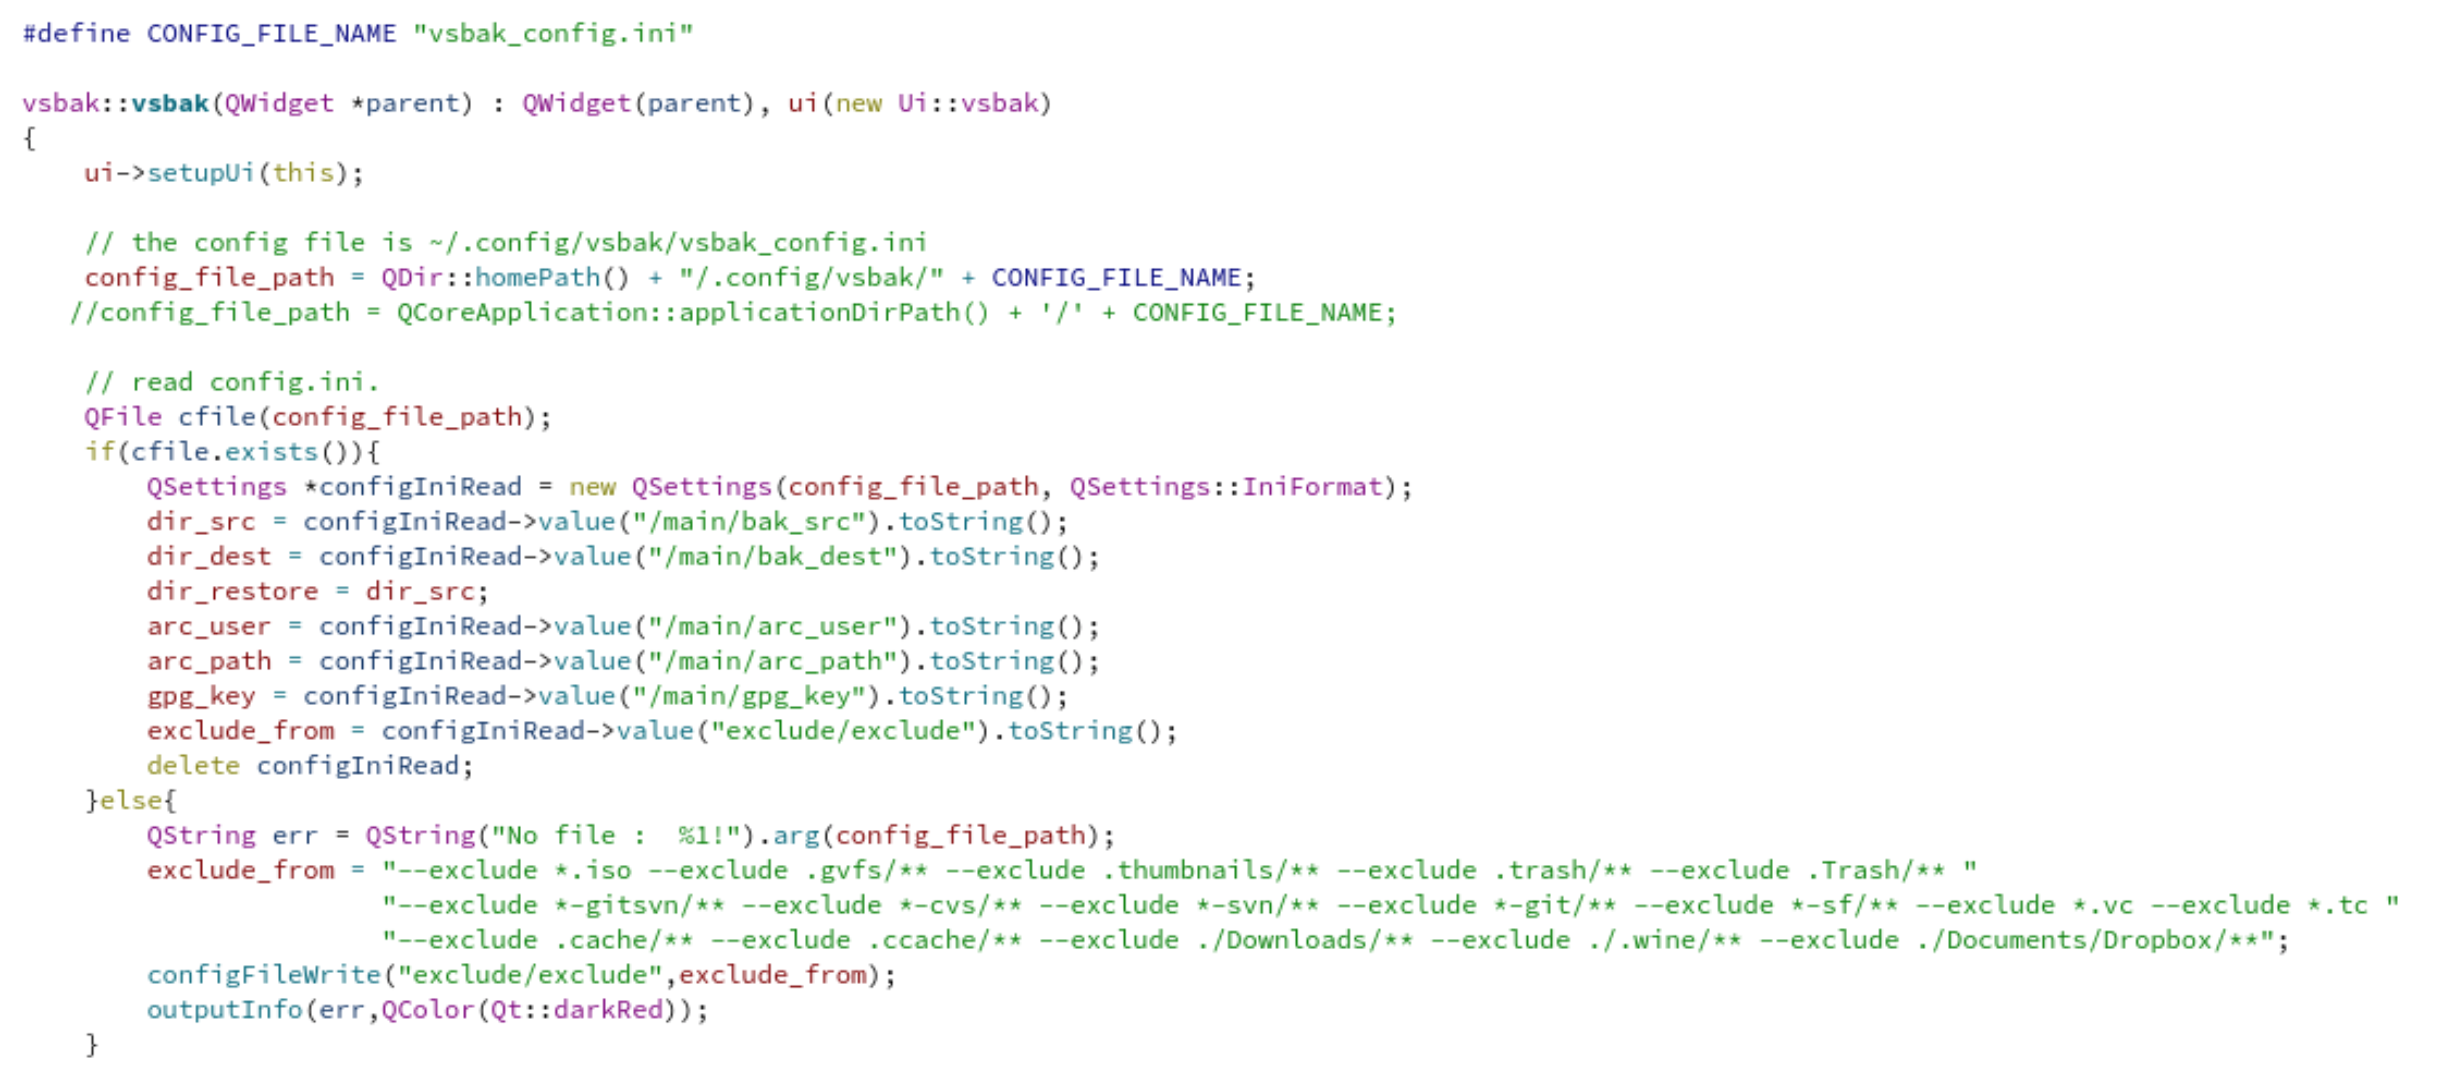
\includegraphics[width=0.9\textwidth]{bilder/code_init_1.png}
	\caption {Der Teil der Initialisierung der Code\_1 }
	\label{Abbildung_18}
\end{figure}


 Vor der Initialisierung wird eine Konfigurationsdatei, die wegen der Initialisierung in einem bestimmten Ort erstellt wird, definiert. In der Initialisierung wird aber durch if-else-Anweisung auch noch bestimmt, ob ein Dokument namens vsbak\_config.ini. existiert. Durch den Zugriff auf die Konfigurationsdatei werden den definierten lokalen Variablen ein paar relevante Informationen wie. z.B. Zieladresse, Quelladresse u.s.w. zugewiesen. Ohne Konfigurationsdatei würde eine Warnung und noch eine Sequenz von Informationen, die die exclude\_from Variable enthaltet,  auf der Benutzeroberfläche angegeben. (s. Abbildung \ref{Abbildung_18})

\begin{figure}[h!]
	\centering
	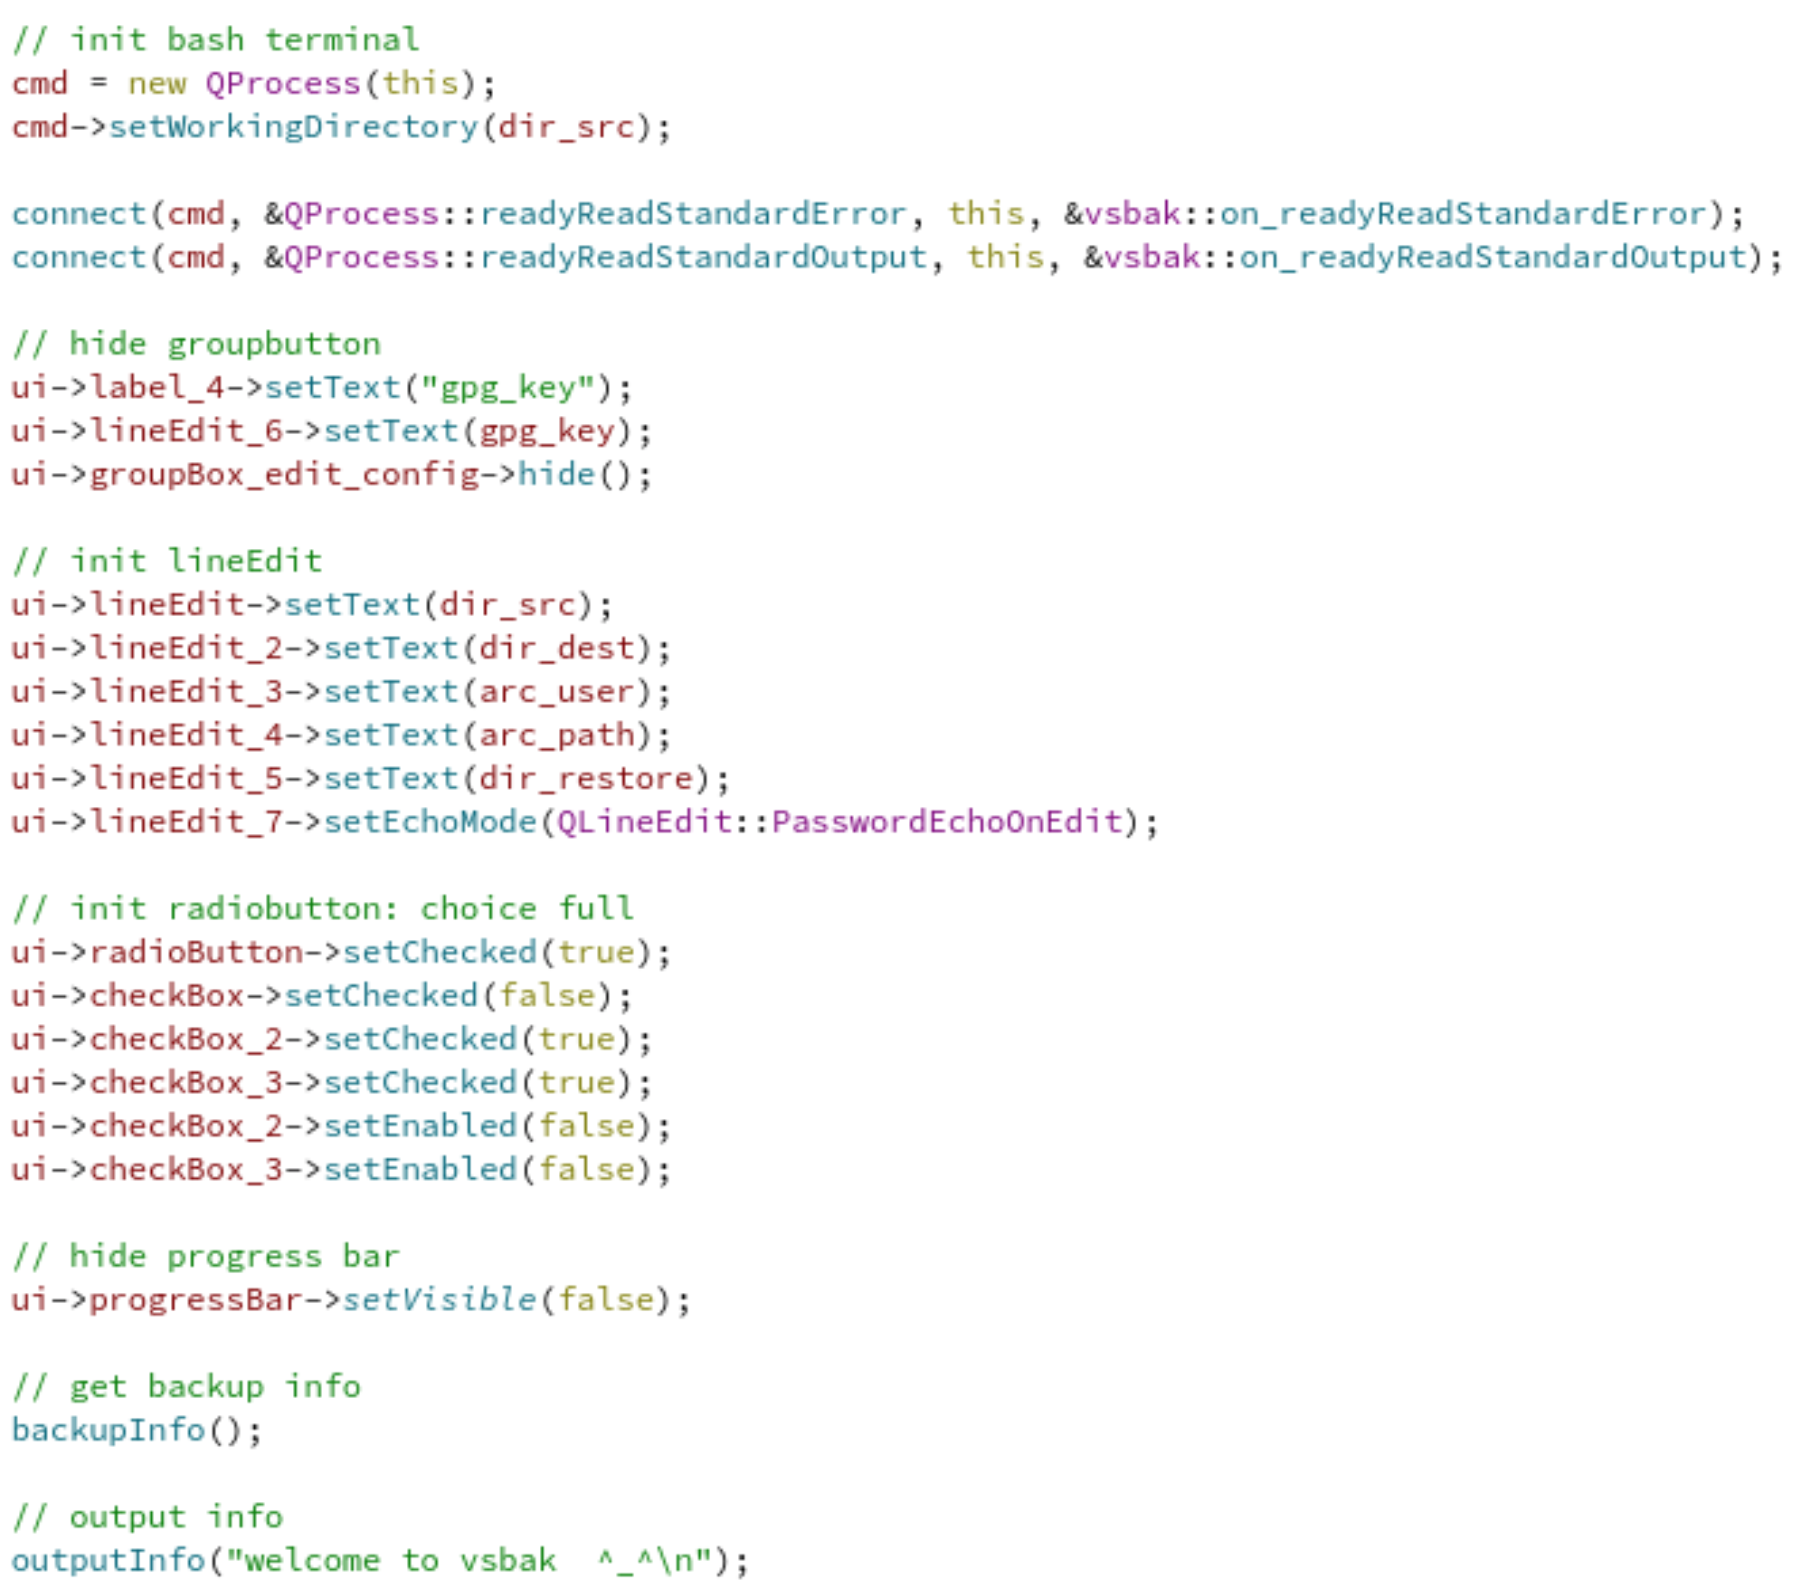
\includegraphics[width=0.9\textwidth]{bilder/code_init_2.png}
	\caption{Der Teil der Initialisierung der Codes2 }
	\label{Abbildung_19}
\end{figure}

\begin{figure}[h!]
	\centering
	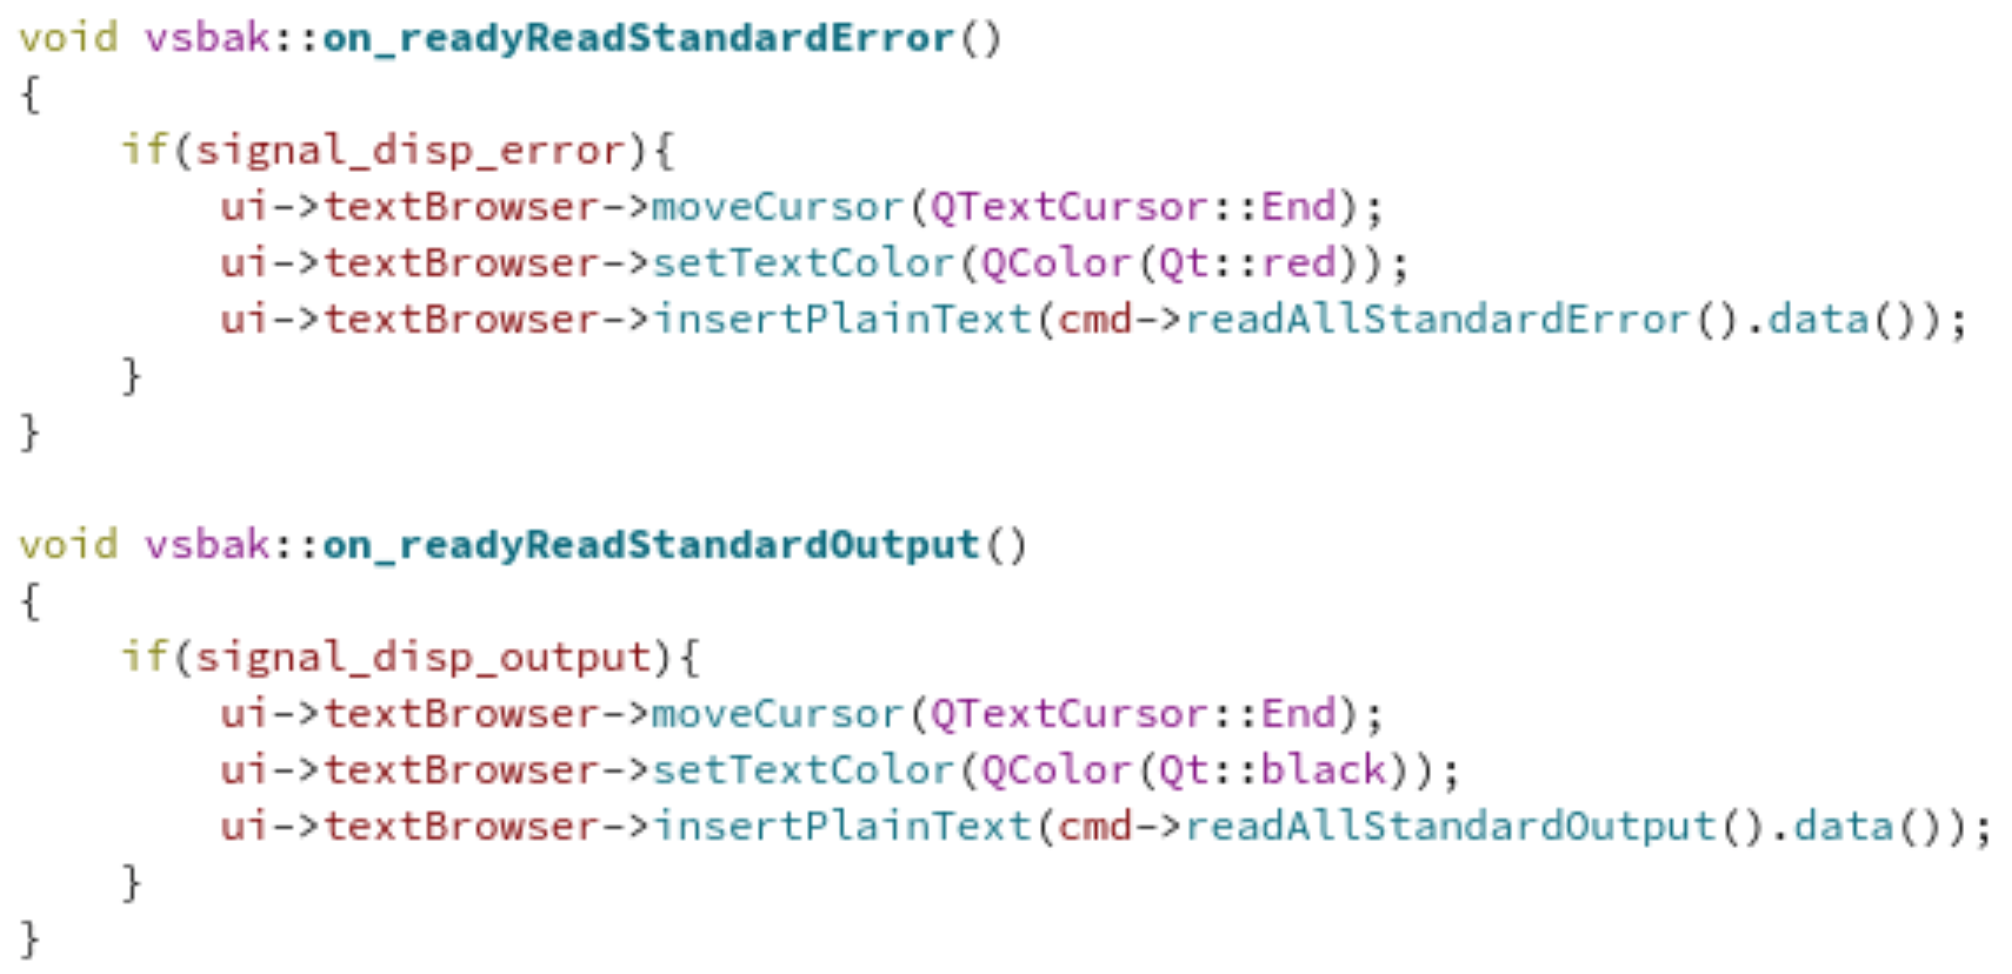
\includegraphics[width=0.9\textwidth]{bilder/code_err_out.png}
	\caption{ on\_readyReadStandardError() und  on\_readyReadStandardOutput() }
	\label{Abbildung_20}
\end{figure}

Darüber hinaus wird ein Objekt der QProcess-Klasse und damit die Quelladresse als die Arbeitsadresse definiert.  Des Weiteren werden zwei Slot-Signal-Paare durch Aufrufe der Connect-Funktion zum Empfang der ausgegebenen Fehler und Ergebnisse des Terminals realisiert, damit die Kommunikation mit Linux-System erfolgreich läuft und sich die Fehler und Ergebnisse auf der grafischen Benutzeroberfläche in TextBrower mit den Funktionen on\_readyReadStandardError() und on\_readyReadStandardOutput() anzeigen lassen. Und was wie z.B. Labels, der anfängliche Zustand des Checkboxes u.s.w. auf der grafischen Benutzeroberfläche festgelegt wird, wird auch dann initialisiert.   Am Ende der Initialisierung wird zweimalige Aufrufe einer selbstdefinierten Funktion geschrieben, um die Backup-Informationen wie z.B. die Informationen einer gebackupten Datei und einen Begrüßungssatz auszugeben. (s. Abbildung \ref{Abbildung_19}  und \ref{Abbildung_20}) 
\par In dem Destruktor wird eine if-Anweisung geschrieben, um einen Prozess völlig zu beenden. 
\par Die in der folgenden Tabelle aufgelisteten Slots-Funktionen werden als Hilfsfunktionen zur Realisierung von Backup, Restore und Upload und einige zusätzliche selbstdefinierte Hilfsfunktionen zur Erleichterung der Bedienung auf der grafischen Benutzeroberfläche aufgebaut. Folglich werden die Hilfsfunktionen und Selbstdefinierten Funktionen und die dazugehörenden Beschreibungen in einer Tabelle aufgeführt.

\begin{table}[h!]
	\caption{Die Slots-Funktion}
	\label{Table1}
	\centering     % 表居中
	\begin{tabular}{|l|l|}
		\hline
		\multicolumn{1}{|c|}{\textbf{Funktion}}    & \multicolumn{1}{c|}{\textbf{Beschreibung}}                                              \\ \hline
		on\_uploadProgress()                       & Ein Hinweis auf den Uploadsprozess.                                                      \\ \hline
		on\_lineEdit\_editingFinished()            &  \makecell[l]{Ein Hinweis auf die erfolgreiche oder erfolglose\\Änderung der Quelladresse.}             \\ \hline
		on\_lineEdit\_2\_editingFinished()         & \makecell[l] {Ein Hinweis auf die erfolgreiche oder erfolglose\\ Änderung der Zieladresse zum Backup}    \\ \hline
		on\_lineEdit\_3\_editingFinished()         &\makecell[l]{Ein Hinweis auf die erfolgreiche oder erfolglose\\ Änderung der Information von arc\_user}  \\ \hline
		on\_lineEdit\_4\_editingFinished()         &\makecell[l]{Ein Hinweis auf die erfolgreiche oder erfolglose \\Änderung der Information von arc\_path}  \\ \hline
		on\_lineEdit\_5\_editingFinished()         & \makecell[l]{Ein Hinweis auf die erfolgreiche oder erfolglose \\Änderung der Adresse zum Restore  }     \\ \hline
		on\_pushButton\_6\_clicked()               & Löschen der gezeigten Inhalte in TestBrowser                                            \\ \hline
		on\_pushButton\_5\_clicked                 & \makecell[l]{Anzeige der detaillierten Informationen von \\Backup}                                      \\ \hline
		on\_pushButton\_4\_clicked()               & Öffnen oder Schließen der Erweiterung                                                   \\ \hline
		on\_pushButton\_9\_clicked()               & Anzeige der Inhalte der Konfigurationsdatei.                                            \\ \hline
		on\_pushButton\_7\_clicked() &\makecell[l]{Wechsel der Funktionen der Erweiterung zur \\Änderung des Schlüsselwortes oder der \\Inhalte in der exclude from-Datei}  \\ \hline
		on\_pushButton\_8\_clicked() &\makecell[l]{Ein Hinweis auf die erfolgreiche Änderung des \\Schlüsselwortes oder der Inhalte in der \\exclude from-Datei} \\ \hline
		on\_toolButton\_clicked()                  & Änderung der Quelladresse                                                               \\ \hline
		on\_toolButton\_2\_clicked()               & Änderung der Zieladresse zum Backup                                                     \\ \hline
		on\_toolButton\_3\_clicked()               & Änderung der Adresse zum Restore                                                        \\ \hline
		on\_checkBox\_clicked()                    & Initialisierung der Checkboxes                                                          \\ \hline
		\begin{tabular}[c]{@{}l@{}}executeCommand(QString line, QString \\command, QStringList argument ,bool \\ sig\_out, bool sig\_err)\end{tabular} &\makecell[l]{Ausführung eines formulierten Linux\\-Kommandos} \\ \hline
		outputInfo(QString out, QColor color)      & Ausgabe der Informationen in den TextBrowser                                            \\ \hline
		configFileWrite(QString path, QString str) & Änderung der Inhalte in der Konfigurationsdatei                                         \\ \hline
	\end{tabular}
\end{table}


Im Weiteren werden die im Programm eine große Rolle spielenden Funktionen als die Hauptfunktionen zur Realisierung von Backup, Restore und Upload analysiert. 
\par on\_pushButton\_clicked() (zum Backup ) \\
on\_pushButton\_2\_clicked() (zum Restore) \\
on\_pushButton\_3\_clicked() (zum Upload)
\par Laut der Aufgabenstellung stellt die Funktion on\_pushButton\_clicked()  die Auswahlen wie die Verschlüsselung, das inkrementelle und vollständige Backup zur Verfügung.  Nach dem Gedankengang wird die Linux-Kommandos zuerst formuliert und bei Bedarf dann ausgeführt werden.
\par Wie in Kapitel 3.1 erwähnt, können die beiden zusätzlichen Auswahlen, nämlich „enc file“ und „tar file“, aber erst willkürlich entfallen oder nicht, nachdem das „encrypting“-Button erstmals ausgewählt werden, weil die beiden nach der Initialisierung angekreuzt werden. Nach der Bestimmung oder Einstellung auf der grafischen Benutzeroberfläche wird im Programm zuerst die Kompression dann die Verschlüsselung ausgeführt.

\begin{figure}[h!]
	\centering
	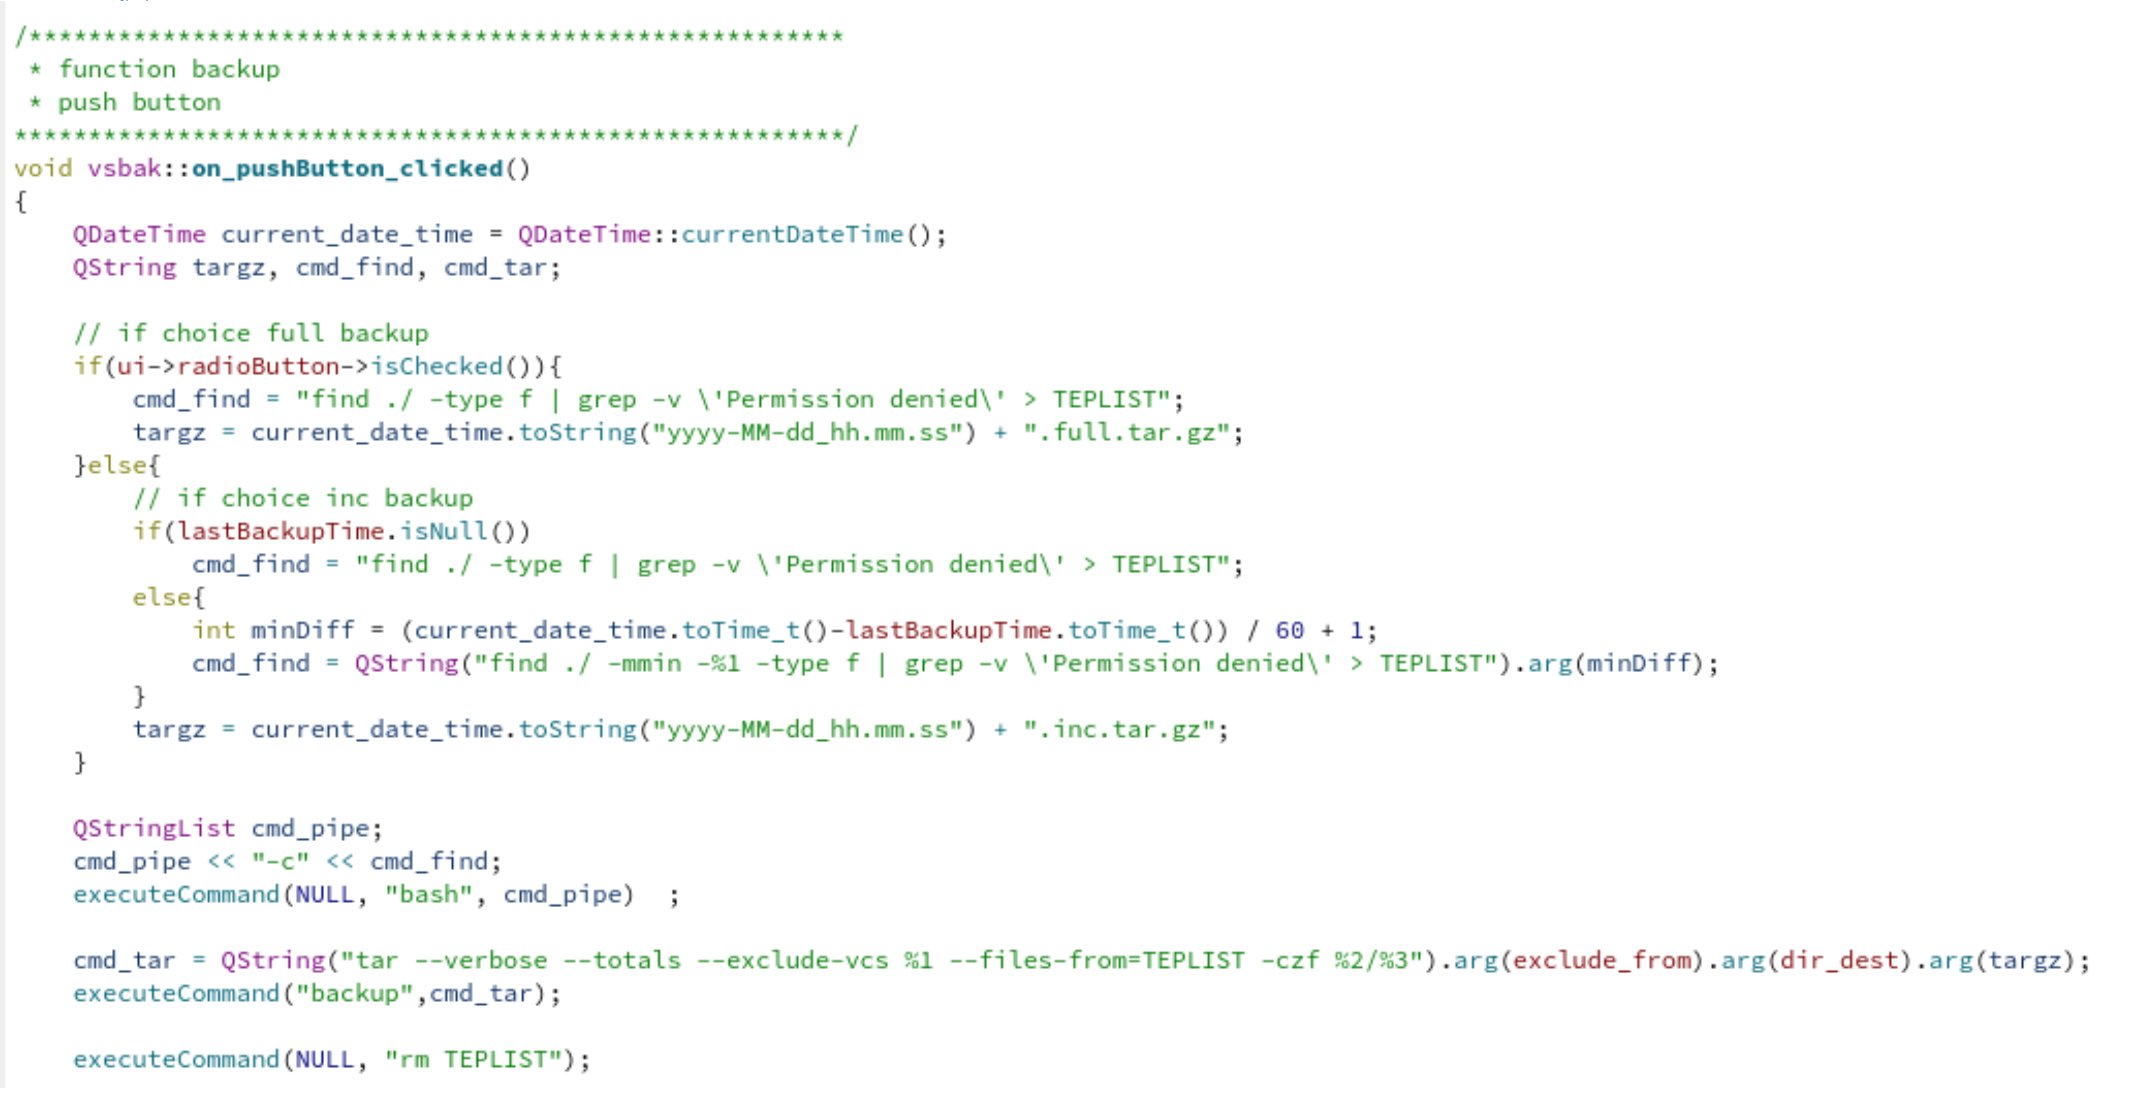
\includegraphics[width=0.9\textwidth]{bilder/code_backup_1.png}
	\caption{ Die Funktion on\_pushButton\_clicked() zum Backup\_1 }
	\label{Abbildung_22}
\end{figure}

In dieser funktion ist ein aktueller Zeitpunkt am Anfang beim Backup bereit. Anschließend wird die Auswahl zwischen dem inkrementellen und vollständigen backup durch eine if-else-Anweisung realisiert. In dem Zweig des sowohl vollständigen als auch inkrementellen backups wird einer Variable ein Linux Kommando in Qstring zugewiesen. Das Kommando sorgt dafür,dass alle Dateien mit dem Zugriffserlaubnis in einem Verzeichnis einer Datei und den dazugehörigen Unterverzeichnisse durch das Linux Kommando bei dem vollständigen Backup ausgewählt und in einer Datei namens „TEPLIST“ aufgelistet werden. Aber im Zweig des inkrementellen Backups werden nur die zuletzt nicht korrigierten oder zugegriffenen Dateien mit Zugriffserlaubnis in „TEPLIST“ aufgelistet. Im Abschluss des Teils wird das Kommando ausgeführt. (s.Abbildung \ref{Abbildung_22})
\par Darüber hinaus wird einer Variable ein Linux Kommando in Qstring zur Kompression einer Datei zugewiesen. Es ist erwähnenswert, dass die in „TEPLIST“ aufgelisteten Dateien ausgeschlossen sind, wenn Sie dem Muster in exclude-from entsprechen. 

\begin{figure}[h!]
	\centering
	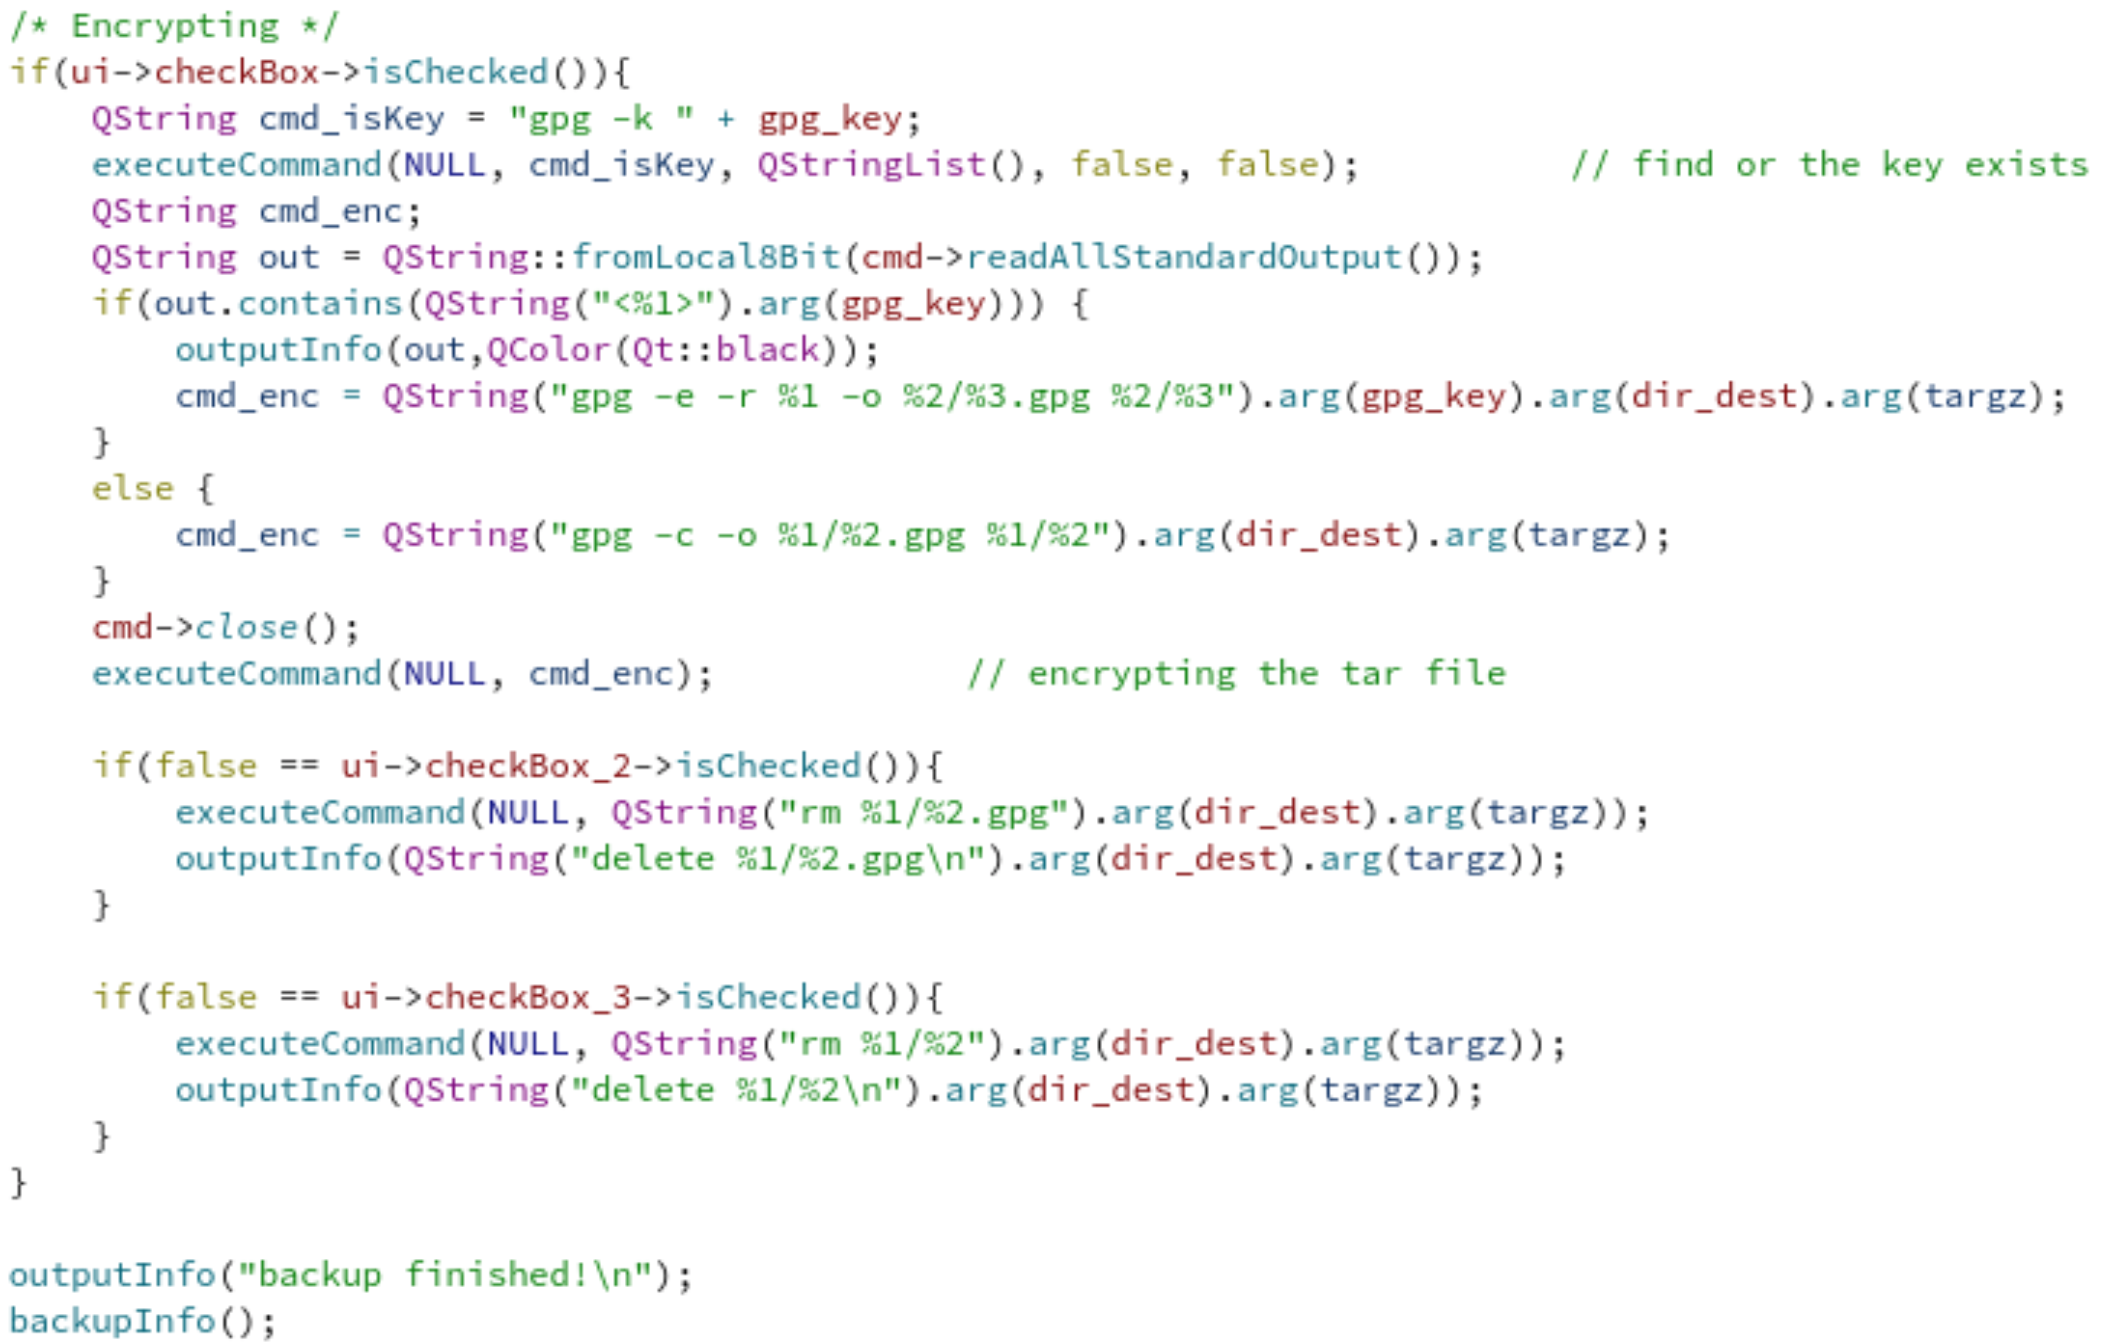
\includegraphics[width=0.9\textwidth]{bilder/code_backup_2.png}
	\caption{ Die Funktion on\_pushButton\_clicked() zum Backup\_2 }
	\label{Abbildung_23}
\end{figure}

In Anschluss an die Codes der Kompression sind die der Verschlüsselung. Am Anfang wird überprüft, ob ein Passwort existiert oder nicht. Wenn ein Passwort vorhanden ist, kann eine Datei direkt verschlüsselt. Wenn kein Passwort, kann eine Datei durch das symmetrische Verschlüsselungsverfahren verschlüsselt. Das Prozess wird mit einer if-else-Anweisung realisiert. Das entsprechende Kommando wird auch einer Variable in QString zugewiesen. 
Am Ende der Funktion wird mit If-else-Anweisung überprüft, ob die Kompression oder Verschlüsselung ausgeführt werden soll. (s.Abbildung \ref{Abbildung_23})

\begin{figure}[h!]
	\centering
	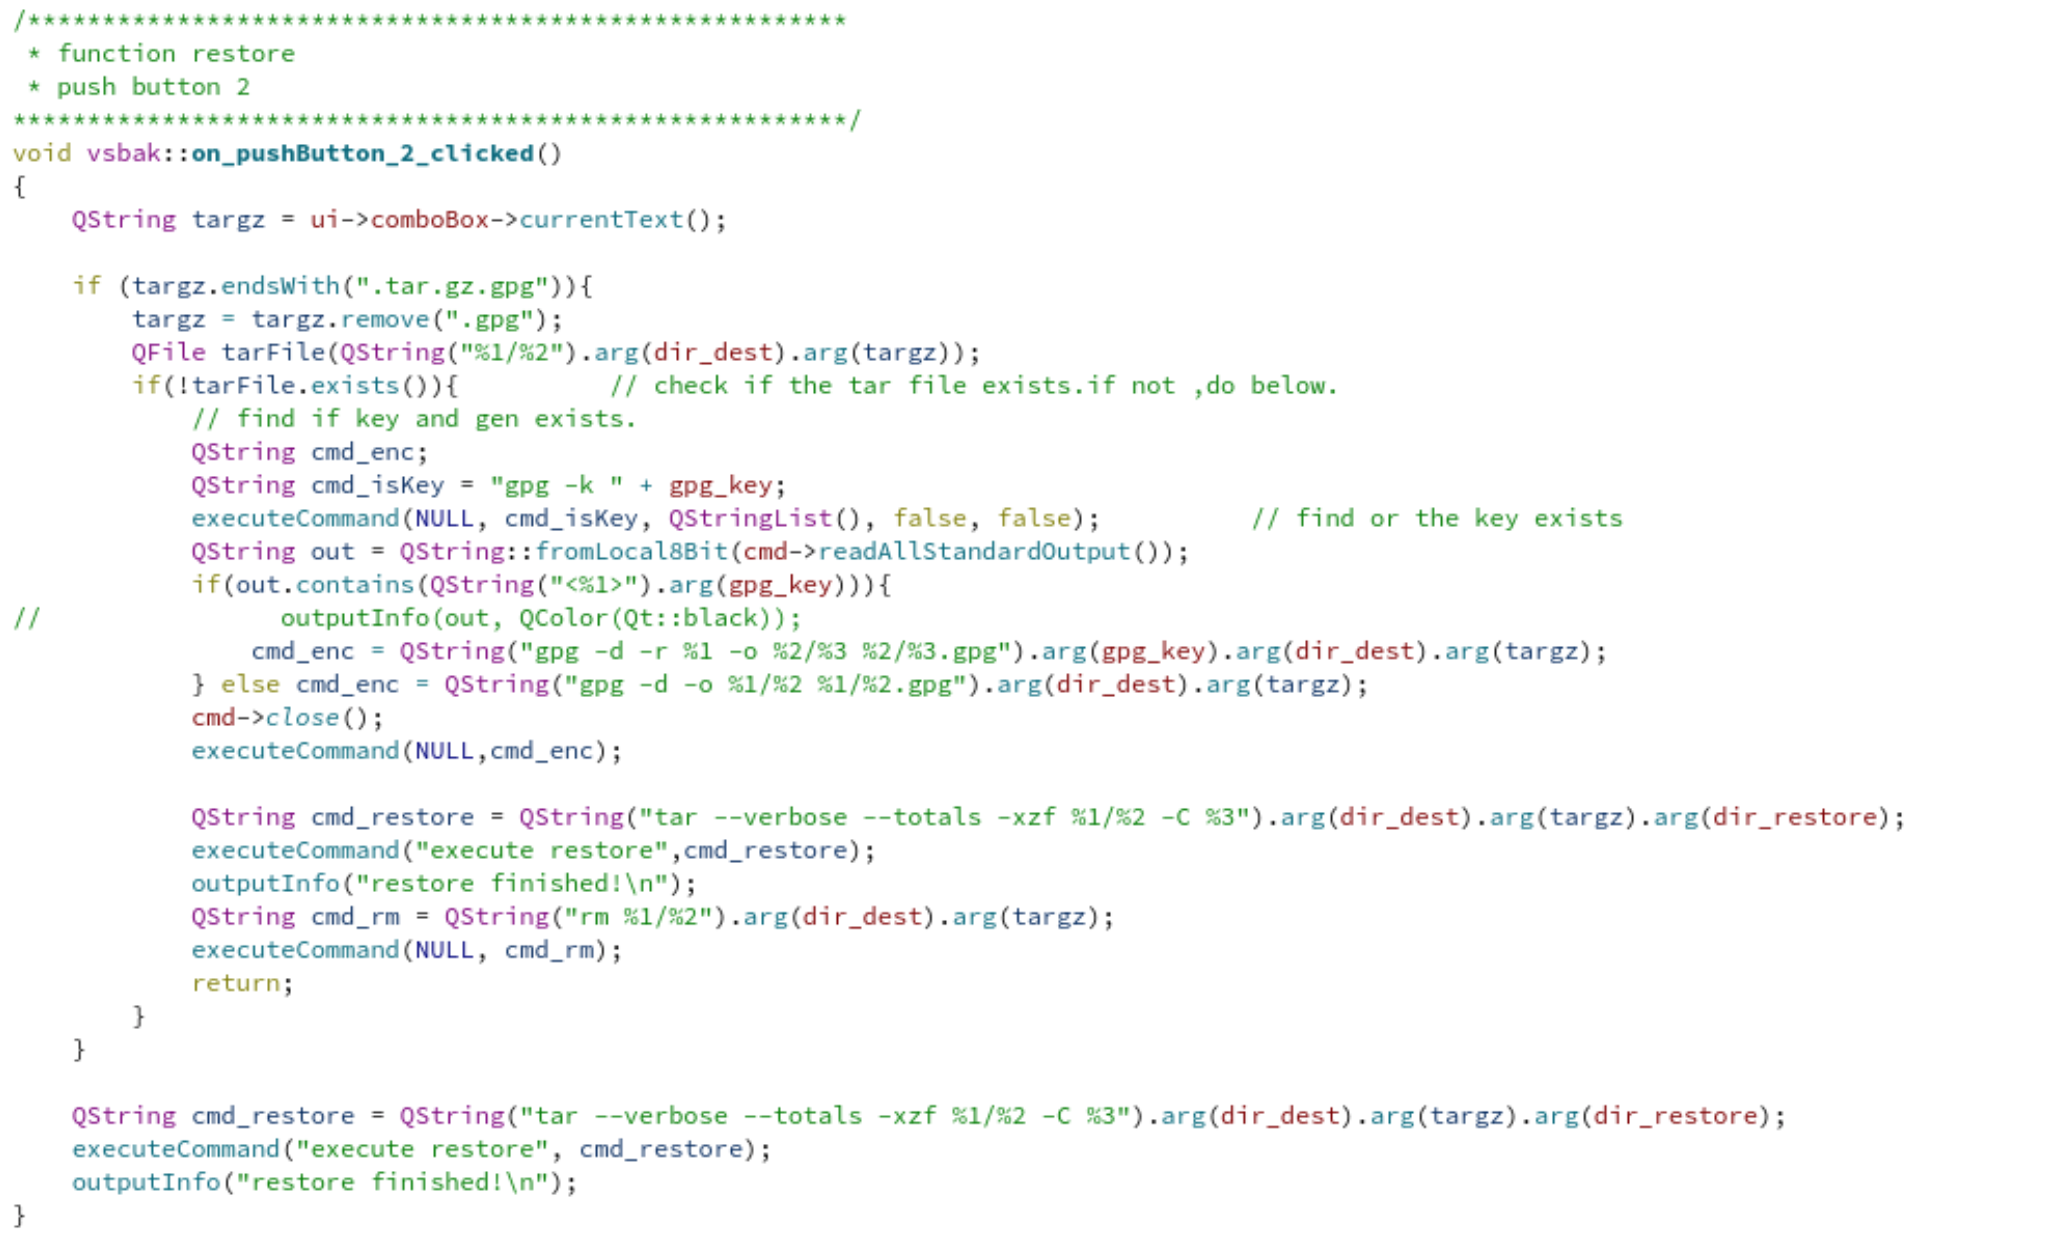
\includegraphics[width=0.9\textwidth]{bilder/code_restore.png}
	\caption{ Die Funktion on\_pushButton\_2\_clicked() zum Restore }
	\label{Abbildung_24}
\end{figure}

In der Funktion on\_pushButton\_2\_clicked() wird erstmals bestimmt, ob eine Datei verschlüsselt. Dann wird die Datei dekomprimiert. Der Prozess ist genau umgekehrt zu dem von der Funktion on\_pushButton\_clicked().(s.Abbildung \ref{Abbildung_24})

\begin{figure}[h!]
	\centering
	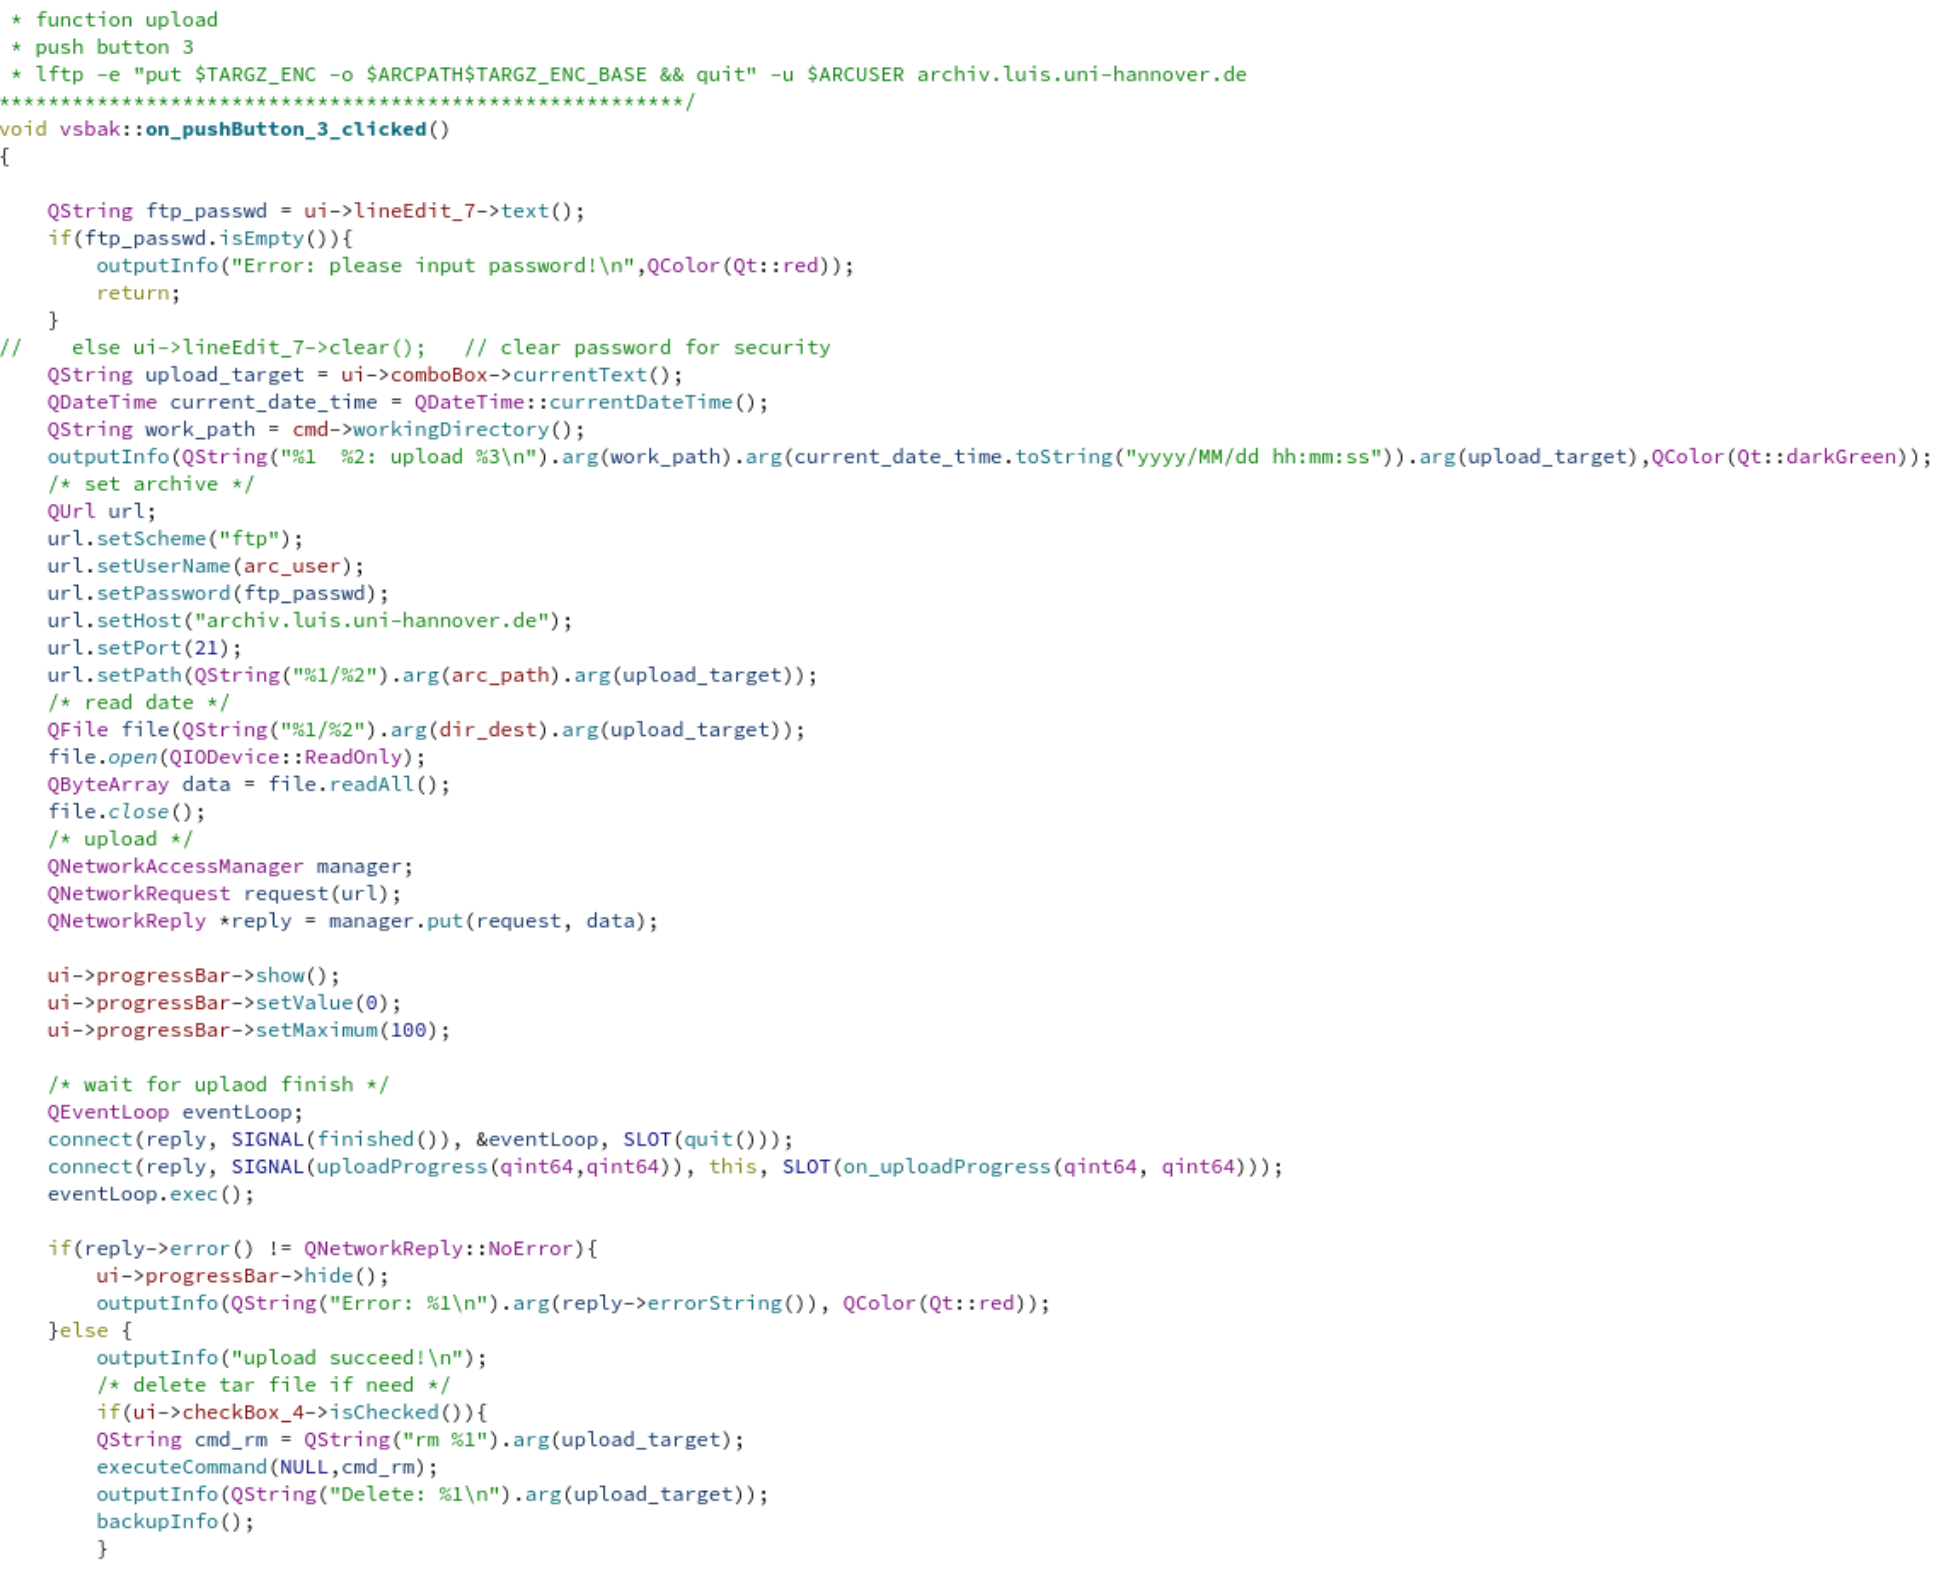
\includegraphics[width=0.9\textwidth]{bilder/code_upload.png}
	\caption{ Die Funktion on\_pushButton\_3\_clicked() zum Upload }
	\label{Abbildung_25}
\end{figure}

Das Dateiübertragungsprotokoll (File Transfer Protocol) wird auf die Funktion on\_pushButton\_3\_clicked() zur Realisierung von Upload angewandt. Zum Beginn wird bestimmt, ob das Passwort eingegeben wird. Anschließend werden die grundsätzlichen Informationen wie die aktuelle Uploadzeit, das dazugehörige Arbeitsverzeichnis und die uploadete Datei auf der grafischen Benutzeroberfläche angezeigt. Dann werden die angeforderten Elemente zum Upload mit dem Dateiübertragungsprotokoll Schritte für Schritte konfiguriert.  Der Hostname lautet „archiv.luis.uni-Hannover.de“.  Außerdem wird ein Fortschrittsbalken durch Aufrufe zweier Connect-Funktionen verwirklicht. (s.Abbildung \ref{Abbildung_25})
